\documentclass[12pt]{IEEEtran}
% Pachete necesare
\usepackage[a4paper, margin=1in]{geometry}
\usepackage{amsmath}
\usepackage{cite}
\usepackage{hyperref}
\usepackage{float}
\usepackage{caption}
\usepackage{tikz}
\usetikzlibrary{arrows.meta, decorations.pathmorphing}
\usepackage{pgfplots}
\pgfplotsset{compat=1.18}

% Titlu, autor, afiliere
\title{Involuntary Cognitive Influence on Quantum Systems: A Hypothesis Based on Human Radar-like Emission}
\author{Teodor Berger,~\IEEEmembership{Independent Researcher}% <-this % stops a space
\thanks{T. Berger is an independent researcher (e-mail: bergerteodor@googlemail.com).}}

\begin{document}

\maketitle

\begin{abstract}
This paper explores the possibility that human cognitive activity may produce involuntary quantum-level effects on physical systems, analogously to echolocation mechanisms in dolphins and bats. We propose that thoughts emit subtle wave-like signals that can interact with quantum particles in a way not yet fully understood, potentially explaining the observer effect. A simplified experimental setup inspired by the double-slit experiment is suggested to test this hypothesis using ordinary participants.
\end{abstract}

\begin{IEEEkeywords}
Quantum mechanics, observer effect, cognitive influence, double-slit experiment, human consciousness
\end{IEEEkeywords}

\section{Introduction}
The quantum observer effect has long puzzled physicists, suggesting that the act of observation can influence the outcome of a quantum event. Traditional interpretations rely on measurement-induced wavefunction collapse. However, we explore a hypothesis wherein mere conscious presence---without deliberate intent---may cause detectable quantum interference.

\section{Biological Analogy: Human Cognitive Radar}
Much like dolphins and bats emit high-frequency signals for spatial awareness, we propose that the human mind emits a form of cognitive ``radar''. This emission is not sonic or electromagnetic in the traditional sense, but rather a currently undefined waveform capable of subtle interaction with quantum systems. This emission ceases or weakens during unconscious states such as sleep or deep meditation.

\section{Hypothesis}
We hypothesize that:
\begin{itemize}
    \item Human cognition emits involuntary signals.
    \item These signals can interfere with quantum particles under certain conditions.
    \item This phenomenon explains part of the observer effect without requiring full consciousness or intent.
\end{itemize}

\section{Proposed Experiment}
A modified double-slit experiment will be used:
\begin{itemize}
    \item A quantum system emits paired particles (e.g., electrons or photons).
    \item A human subject, unaware of the timing, is placed nearby.
    \item The interference pattern is recorded both with and without the human's presence.
    \item Variations are analyzed to detect statistical deviation consistent with wave interference.
\end{itemize}

\begin{figure}[!t]
\centering
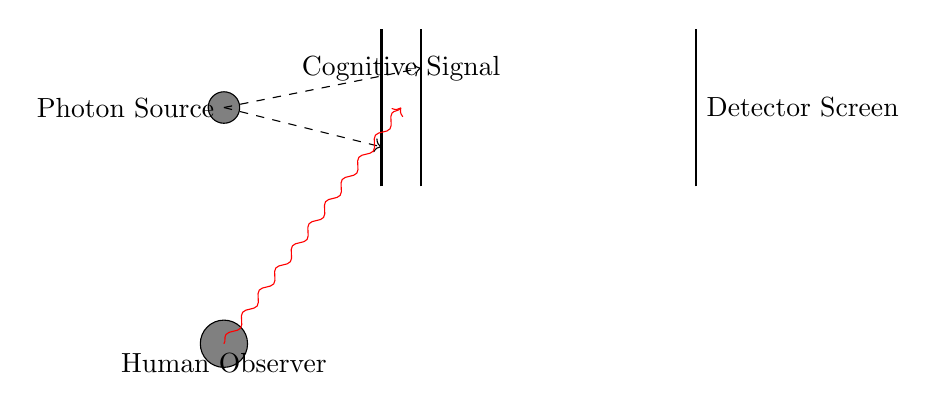
\begin{tikzpicture}
    % Slits
    \draw[thick] (0,0) -- (0,2);
    \draw[thick] (0.5,0) -- (0.5,2);
    % Photon source
    \draw[fill=gray] (-2,1) circle (0.2) node[left] {Photon Source};
    % Detector screen
    \draw[thick] (4,0) -- (4,2) node[midway, right] {Detector Screen};
    % Human observer
    \draw[fill=gray] (-2,-2) circle (0.3) node[below] {Human Observer};
    % Photon paths
    \draw[->, dashed] (-2,1) -- (0,0.5);
    \draw[->, dashed] (-2,1) -- (0.5,1.5);
    % Cognitive signal
    \draw[->, red, decorate, decoration={snake, amplitude=0.5mm}] (-2,-2) -- (0.25,1);
    \node at (0.25,1.5) {Cognitive Signal};
\end{tikzpicture}
\caption{Schematic of the experimental setup: a human observer emits cognitive signals that may interact with photons passing through slits, influencing the interference pattern. See Appendix~\ref{app:figures} for the complete code.}
\label{fig:setup}
\end{figure}

\section{Methodology}
To rigorously test the hypothesis, we outline a detailed experimental protocol.

\subsection{Experimental Setup}
A double-slit apparatus is configured to emit paired photons generated via spontaneous parametric down-conversion. The slits are spaced 0.1 mm apart, with a detector screen positioned 1 m away. The human subject is seated 2 m from the slits, facing the apparatus but unaware of the photon emission timing to minimize intentional influence.

\subsection{Control Conditions}
Two conditions are tested:
\begin{itemize}
    \item \textbf{Presence}: The subject is awake and present during photon emission.
    \item \textbf{Absence}: No human subject is present, or the subject is in a meditative state to suppress cognitive activity.
\end{itemize}
Each condition is repeated for 1000 trials to ensure statistical significance.

\subsection{Error Sources}
Potential sources of error include:
\begin{itemize}
    \item \textbf{Mental noise}: Random cognitive activity may introduce variability.
    \item \textbf{Environmental interference}: Electromagnetic fluctuations or temperature variations may affect the apparatus.
    \item \textbf{Subject fatigue}: Prolonged exposure may alter cognitive emission strength.
\end{itemize}
These are mitigated by shielding the setup, maintaining consistent environmental conditions, and limiting session duration.

\subsection{Data Analysis}
The interference pattern is recorded as a histogram of photon detection positions. We compute the standard deviation of the interference fringes and apply a two-sample t-test to compare the presence and absence conditions. A p-value threshold of 0.05 is used to determine significance.

\subsection{Expected Outcomes}
If the hypothesis holds, the presence condition should exhibit a statistically significant deviation in the interference pattern compared to the absence condition, suggesting an involuntary cognitive influence.

\section{Numerical Simulation}
To illustrate the expected effect, we simulate the interference pattern using a cosine-squared model perturbed by a constant offset to represent cognitive influence. The simulation code is available in the accompanying repository at \url{https://github.com/DonMask/QuantumCognitiveRadar} (see file \texttt{simulation.py}). The resulting plot (see Fig.~\ref{fig:interference}) shows a clear deviation in the interference pattern when the observer is present. The dataset and code are archived at \href{https://doi.org/10.5281/zenodo.15458571}{Zenodo (DOI: 10.5281/zenodo.15458571)}.

\begin{figure}[!t]
\centering
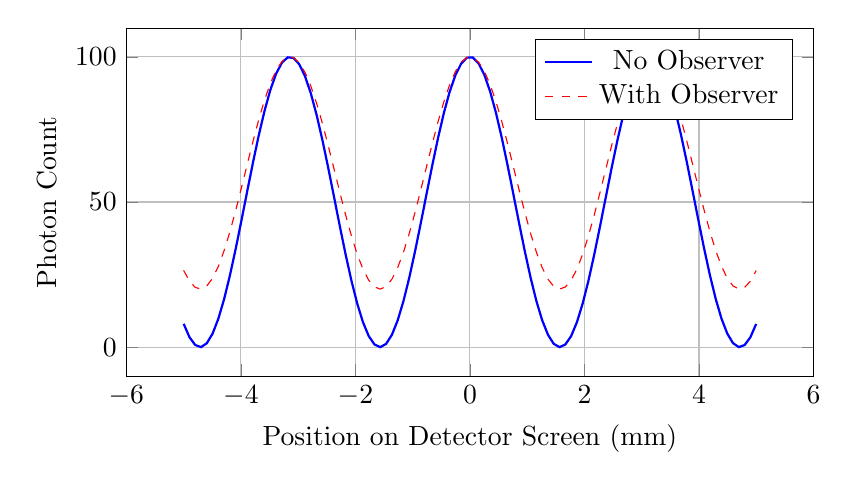
\begin{tikzpicture}
\begin{axis}[
    xlabel={Position on Detector Screen (mm)},
    ylabel={Photon Count},
    domain=-5:5,
    samples=100,
    width=0.85\textwidth,
    height=6cm,
    grid=major,
    legend pos=north east
]
    % Interference pattern without observer
    \addplot[blue, thick] {100*(cos(deg(x)))^2};
    \addlegendentry{No Observer}
    % Interference pattern with observer
    \addplot[red, dashed] {80*(cos(deg(x)))^2 + 20};
    \addlegendentry{With Observer}
\end{axis}
\end{tikzpicture}
\caption{Expected interference patterns: the blue curve represents the pattern without a human observer, while the red dashed curve shows a hypothesized deviation due to cognitive influence. See Appendix~\ref{app:figures} for the complete code.}
\label{fig:interference}
\end{figure}

\section{Mathematical Model}
The interference pattern is modeled as a superposition of wavefunctions from two slits. The probability density of photon detection is given by:
\begin{equation}
P(x) = \left| \psi_1(x) + \psi_2(x) \right|^2,
\end{equation}
where \(\psi_1(x)\) and \(\psi_2(x)\) are the wavefunctions from each slit. We hypothesize that the cognitive signal introduces a phase shift \(\phi\), modifying the probability to:
\begin{equation}
P'(x) = \left| \psi_1(x)e^{i\phi} + \psi_2(x) \right|^2.
\end{equation}
This shift is expected to alter the interference fringes, detectable via statistical analysis.

\section{Discussion}
The process appears to be automatic, possibly evolutionary in nature. It does not require understanding or focus, much like echolocation is instinctive in animals. This interpretation re-frames the observer effect as a natural consequence of incomplete biological evolution, rather than purely a philosophical paradox.

Potential applications include improving quantum detection equipment by accounting for cognitive interference, or exploring neuroscientific studies to quantify the strength and nature of cognitive emissions. For instance, such findings could inform the design of quantum sensors used in medical imaging or enhance our understanding of consciousness in cognitive science.

\section{Conclusion}
The mind may function as a radar-like emitter, influencing quantum events without deliberate observation. If proven, this insight could deepen our understanding of consciousness, measurement, and quantum mechanics.

\section*{References}
\bibliographystyle{IEEEtran}
\bibliography{references}

\appendices
\section{Figure Code}
\label{app:figures}
The following LaTeX code generates the figures in this paper.

\subsection{Experimental Setup (Fig.~\ref{fig:setup})}
\begin{verbatim}
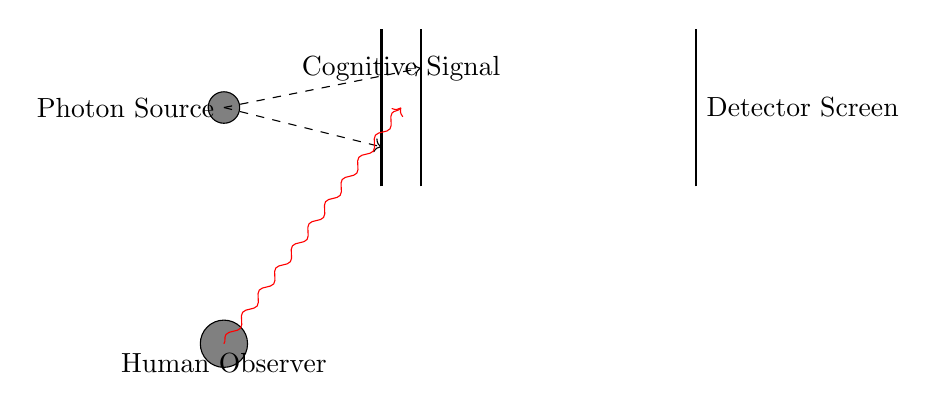
\begin{tikzpicture}
    % Slits
    \draw[thick] (0,0) -- (0,2);
    \draw[thick] (0.5,0) -- (0.5,2);
    % Photon source
    \draw[fill=gray] (-2,1) circle (0.2) node[left] {Photon Source};
    % Detector screen
    \draw[thick] (4,0) -- (4,2) node[midway, right] {Detector Screen};
    % Human observer
    \draw[fill=gray] (-2,-2) circle (0.3) node[below] {Human Observer};
    % Photon paths
    \draw[->, dashed] (-2,1) -- (0,0.5);
    \draw[->, dashed] (-2,1) -- (0.5,1.5);
    % Cognitive signal
    \draw[->, red, decorate, decoration={snake, amplitude=0.5mm}] (-2,-2) -- (0.25,1);
    \node at (0.25,1.5) {Cognitive Signal};
\end{tikzpicture}
\end{verbatim}

\subsection{Interference Patterns (Fig.~\ref{fig:interference})}
\begin{verbatim}
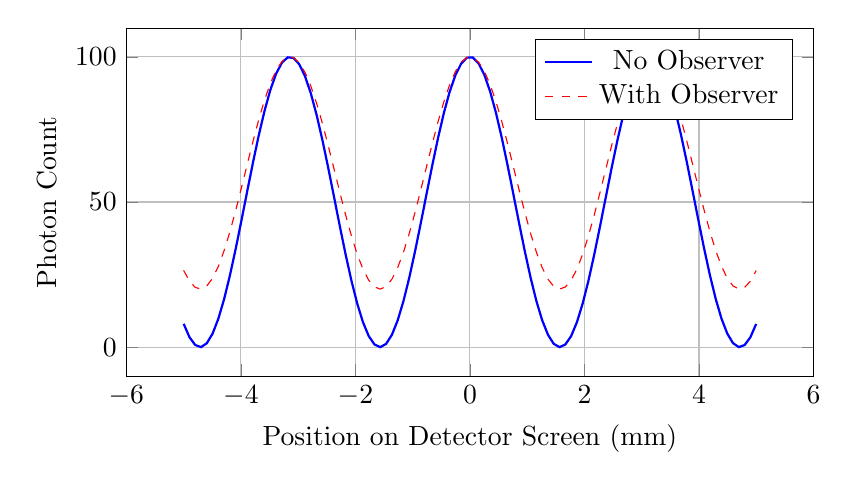
\begin{tikzpicture}
\begin{axis}[
    xlabel={Position on Detector Screen (mm)},
    ylabel={Photon Count},
    domain=-5:5,
    samples=100,
    width=0.85\textwidth,
    height=6cm,
    grid=major,
    legend pos=north east
]
    \addplot[blue, thick] {100*(cos(deg(x)))^2};
    \addlegendentry{No Observer}
    \addplot[red, dashed] {80*(cos(deg(x)))^2 + 20};
    \addlegendentry{With Observer}
\end{axis}
\end{tikzpicture}
\end{verbatim}

\end{document}
